% Document principal LaTeX pour compte-rendu
\documentclass{article}
\usepackage{graphicx}
\usepackage{tikz}




\begin{document}

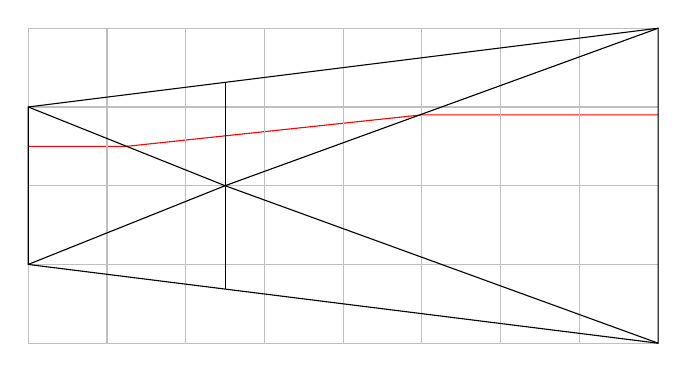
\begin{tikzpicture}
    \coordinate (A) at (0,0);
    \coordinate (B) at (8,-1);
    \coordinate (C) at (8,3);
    \coordinate (D) at (0,2);
    \coordinate (E) at (2.5, 1);
    \coordinate (F) at (2.5, 2.31);
    \coordinate (G) at (2.5, -0.31);
    \coordinate (H) at (0, 1.5);
    \coordinate (I) at (1.25, 1.5);
    \coordinate (J) at (5, 1.9);
    \coordinate (K) at (8, 1.9);
    
    \draw[color=red] (H) -- (I) -- (J) -- (K);
    \draw[color=lightgray] (0, 3) -- (0, -1);
    \draw[color=lightgray] (1, 3) -- (1, -1);
    \draw[color=lightgray] (2, 3) -- (2, -1);
    \draw[color=lightgray] (3, 3) -- (3, -1);
    \draw[color=lightgray] (4, 3) -- (4, -1);
    \draw[color=lightgray] (5, 3) -- (5, -1);
    \draw[color=lightgray] (6, 3) -- (6, -1);
    \draw[color=lightgray] (7, 3) -- (7, -1);
    \draw[color=lightgray] (8, 3) -- (8, -1);
    \draw[color=lightgray] (0, 3) -- (8, 3);
    \draw[color=lightgray] (0, 2) -- (8, 2);
    \draw[color=lightgray] (0, 1) -- (8, 1);   
    \draw[color=lightgray] (0, 0) -- (8, 0);
    \draw[color=lightgray] (0, -1) -- (8, -1);

    \draw (A) -- (B) -- (C) -- (D) -- cycle;
    \draw (A) -- (E) -- (C);
    \draw (D) -- (E) -- (B);
    \draw (F) -- (E) -- (G);
    
    % \node[below left] at (A) {A};
    % \node[below right] at (B) {B};
    % \node[above right] at (C) {C};
    % \node[above left] at (D) {D};
    % \node[above left] at (E) {E};
    % \node[above right] at (F) {F};
    % \node[above left] at (G) {G};
    % \node[above right] at (H) {H};
    % \node[above right] at (I) {I};
    % \node[above right] at (J) {J};
\end{tikzpicture}

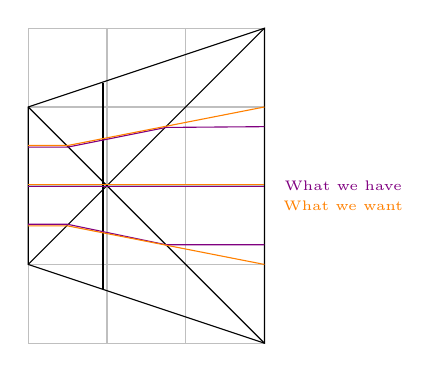
\begin{tikzpicture}
    \coordinate (A) at (0,0);
    \coordinate (B) at (3,-1);
    \coordinate (C) at (3,3);
    \coordinate (D) at (0,2);
    \coordinate (E) at (0.95, -0.31);
    \coordinate (F) at (0.95, 2.31);
    
    \draw[color=lightgray] (0, 3) -- (0, -1);
    \draw[color=lightgray] (1, 3) -- (1, -1);
    \draw[color=lightgray] (2, 3) -- (2, -1);
    \draw[color=lightgray] (3, 3) -- (3, -1);
    \draw[color=lightgray] (0, 3) -- (3, 3);
    \draw[color=lightgray] (0, 2) -- (3, 2);
    \draw[color=lightgray] (0, 1) -- (3, 1);   
    \draw[color=lightgray] (0, 0) -- (3, 0);
    \draw[color=lightgray] (0, -1) -- (3, -1);

    \draw (A) -- (B) -- (C) -- (D) -- cycle;
    \draw (A) -- (C);
    \draw (B) -- (D);
    \draw (F) -- (E);

    \draw[color=violet] (0, 1.49) -- (0.5, 1.49) -- (1.75 , 1.74) -- (3, 1.75);
    \draw[color=orange] (0, 1.51) -- (0.5, 1.51) -- (3, 2);

    \draw[color=violet] (0, 0.99) -- (3, 0.99);
    \draw[color=orange] (0, 1.01) -- (3, 1.01);

    \draw[color=violet] (0, 0.51) -- (0.5, 0.51) -- (1.75 , 0.25) -- (3, 0.25);
    \draw[color=orange] (0, 0.49) -- (0.5, 0.49) -- (3, 0);

    % Écriture de texte de couleur
    \node[color=violet] at (4, 1) {\tiny What we have};
    \node[color=orange] at (4, 0.75) {\tiny What we want};

    % \node[below left] at (A) {A};
    % \node[below right] at (B) {B};
    % \node[above right] at (C) {C};
    % \node[above left] at (D) {D};
    % \node[above left] at (E) {E};
    % \node[above right] at (F) {F};
\end{tikzpicture}

    
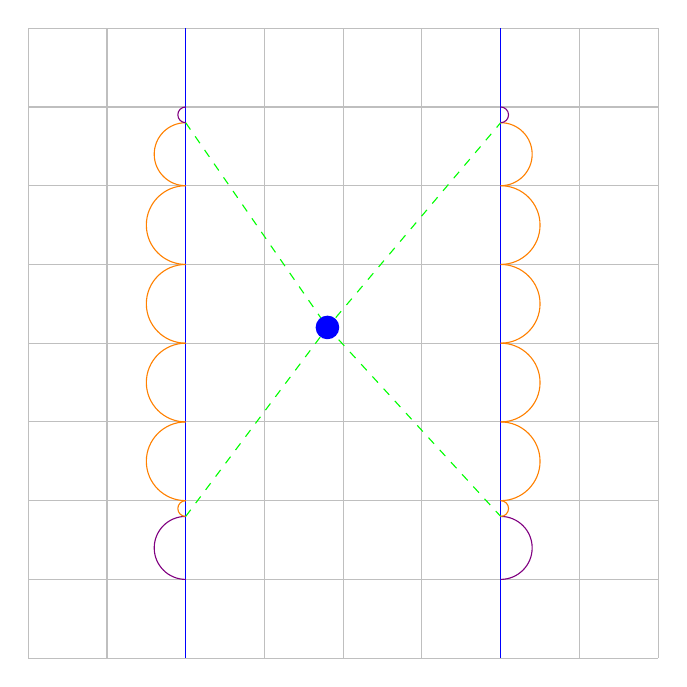
\begin{tikzpicture}

    Factoriser le segement à afficher pour mettre une texture sur chaque section

    \draw[color=lightgray] (0, 8) -- (0, 0);
    \draw[color=lightgray] (1, 8) -- (1, 0);
    \draw[color=lightgray] (2, 8) -- (2, 0);
    \draw[color=lightgray] (3, 8) -- (3, 0);
    \draw[color=lightgray] (4, 8) -- (4, 0);
    \draw[color=lightgray] (5, 8) -- (5, 0);
    \draw[color=lightgray] (6, 8) -- (6, 0);
    \draw[color=lightgray] (7, 8) -- (7, 0);
    \draw[color=lightgray] (8, 8) -- (8, 0);

    \draw[color=lightgray] (0, 8) -- (8, 8);
    \draw[color=lightgray] (0, 7) -- (8, 7);
    \draw[color=lightgray] (0, 6) -- (8, 6);
    \draw[color=lightgray] (0, 5) -- (8, 5);
    \draw[color=lightgray] (0, 4) -- (8, 4);
    \draw[color=lightgray] (0, 3) -- (8, 3);
    \draw[color=lightgray] (0, 2) -- (8, 2);
    \draw[color=lightgray] (0, 1) -- (8, 1);   
    \draw[color=lightgray] (0, 0) -- (8, 0);

    \draw[color=blue] (2, 0) -- (2, 8);
    \draw[color=blue] (6, 0) -- (6, 8);

    \draw[dashed, color=green] (2, 6.8) -- (3.8, 4.2) -- (6, 1.8);
    \draw[dashed, color=green] (2, 1.8) -- (3.8, 4.2) -- (6, 6.8);

    \fill[blue] (3.8, 4.2) circle (0.15);

    \draw[color=violet] (2,1.8) arc (-90:90:-0.4);

    \draw[color=orange] (2,2) arc (-90:90:-0.1);
    \draw[color=orange] (2,3) arc (-90:90:-0.5);
    \draw[color=orange] (2,4) arc (-90:90:-0.5);
    \draw[color=orange] (2,5) arc (-90:90:-0.5);
    \draw[color=orange] (2,6) arc (-90:90:-0.5);
    \draw[color=orange] (2,6.8) arc (-90:90:-0.4);

    \draw[color=violet] (2,7) arc (-90:90:-0.1);


    \draw[color=violet] (6,1.8) arc (90:-90:0.4);

    \draw[color=orange] (6,2) arc (90:-90:0.1);
    \draw[color=orange] (6,3) arc (90:-90:0.5);
    \draw[color=orange] (6,4) arc (90:-90:0.5);
    \draw[color=orange] (6,5) arc (90:-90:0.5);
    \draw[color=orange] (6,6) arc (90:-90:0.5);
    \draw[color=orange] (6,6.8) arc (90:-90:0.4);

    \draw[color=violet] (6,7) arc (90:-90:0.1);

\end{tikzpicture}

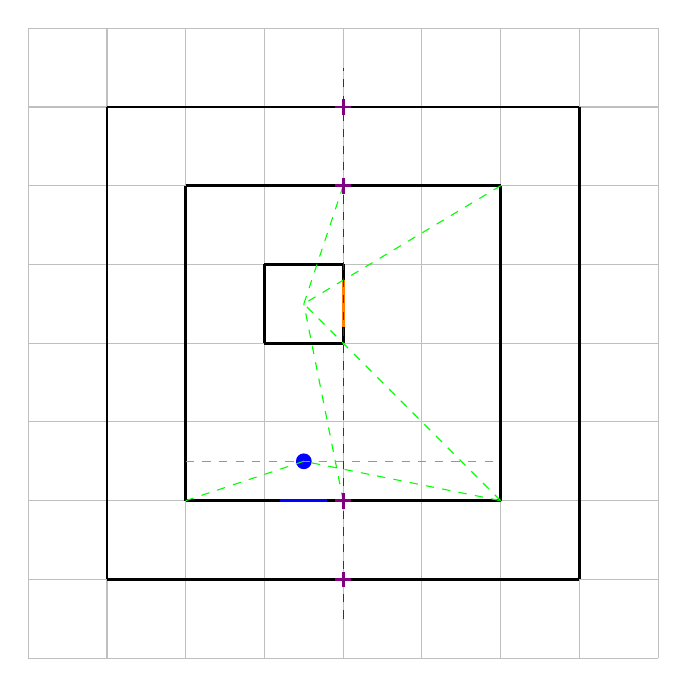
\begin{tikzpicture}

    \draw[color=lightgray] (0, 8) -- (0, 0);
    \draw[color=lightgray] (1, 8) -- (1, 0);
    \draw[color=lightgray] (2, 8) -- (2, 0);
    \draw[color=lightgray] (3, 8) -- (3, 0);
    \draw[color=lightgray] (4, 8) -- (4, 0);
    \draw[color=lightgray] (5, 8) -- (5, 0);
    \draw[color=lightgray] (6, 8) -- (6, 0);
    \draw[color=lightgray] (7, 8) -- (7, 0);
    \draw[color=lightgray] (8, 8) -- (8, 0);

    \draw[color=lightgray] (0, 8) -- (8, 8);
    \draw[color=lightgray] (0, 7) -- (8, 7);
    \draw[color=lightgray] (0, 6) -- (8, 6);
    \draw[color=lightgray] (0, 5) -- (8, 5);
    \draw[color=lightgray] (0, 4) -- (8, 4);
    \draw[color=lightgray] (0, 3) -- (8, 3);
    \draw[color=lightgray] (0, 2) -- (8, 2);
    \draw[color=lightgray] (0, 1) -- (8, 1);   
    \draw[color=lightgray] (0, 0) -- (8, 0);

    \draw[line width=1pt] (1, 1) -- (1, 7);
    \draw[line width=1pt] (1, 1) -- (7, 1);
    \draw[line width=1pt] (7, 1) -- (7, 7);
    \draw[line width=1pt] (1, 7) -- (7, 7);

    \draw[line width=1pt] (2, 2) -- (2, 6);
    \draw[line width=1pt] (2, 2) -- (6, 2);
    \draw[line width=1pt] (6, 2) -- (6, 6);
    \draw[line width=1pt] (2, 6) -- (6, 6);

    \draw[line width=1pt] (3, 5) -- (4, 5);
    \draw[line width=1pt] (3, 4) -- (4, 4);
    \draw[line width=1pt] (3, 5) -- (3, 4);
    \draw[line width=1pt] (4, 5) -- (4, 4);

    \draw[line width=1pt, color=blue] (3.2, 2) -- (3.8, 2);

    \draw[line width=1pt, color=orange] (4, 4.2) -- (4, 4.8);

    \fill[blue] (3.5, 2.5) circle (0.1);

    \draw[color=green, dashed] (2, 2) -- (3.5, 2.5) -- (6, 2);
    \draw[color=green, dashed] (2, 2.5) -- (3.5, 2.5) -- (6, 2.5);
    \draw[color=green, dashed] (6, 2) -- (3.5, 4.5);
    \draw[color=green, dashed] (6, 6) -- (3.5, 4.5);
    \draw[color=green, dashed] (4, 6) -- (3.5, 4.5);
    \draw[color=green, dashed] (4, 2) -- (3.5, 4.5);

    \draw[color=violet, dashed] (4, 0.5) -- (4, 7.5);
    \draw[color=violet, line width=1pt] (4, 0.9) -- (4, 1.1);
    \draw[color=violet, line width=1pt] (3.9, 1) -- (4.1, 1);

    \draw[color=violet, line width=1pt] (4, 1.9) -- (4, 2.1);
    \draw[color=violet, line width=1pt] (3.9, 2) -- (4.1, 2);

    \draw[color=violet, line width=1pt] (4, 5.9) -- (4, 6.1);
    \draw[color=violet, line width=1pt] (3.9, 6) -- (4.1, 6);

    \draw[color=violet, line width=1pt] (4, 6.9) -- (4, 7.1);
    \draw[color=violet, line width=1pt] (3.9, 7) -- (4.1, 7);

    
\end{tikzpicture}

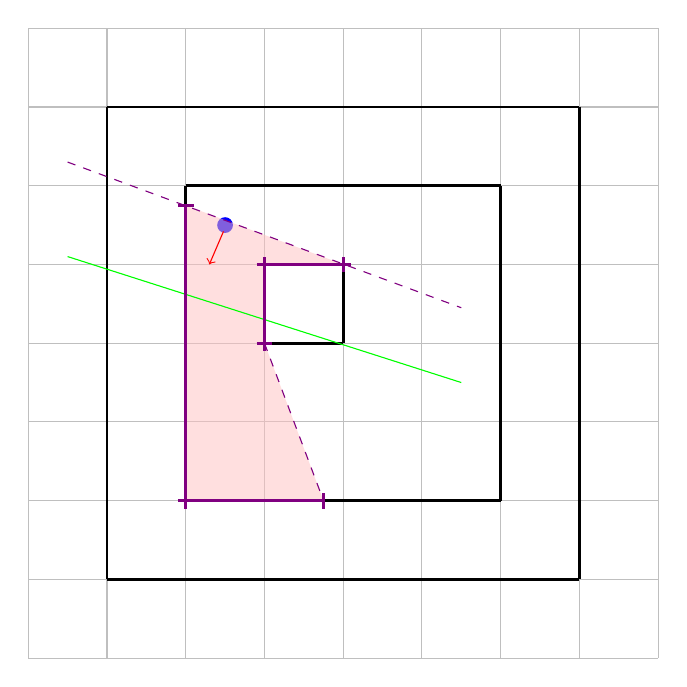
\begin{tikzpicture}

    \draw[color=lightgray] (0, 8) -- (0, 0);
    \draw[color=lightgray] (1, 8) -- (1, 0);
    \draw[color=lightgray] (2, 8) -- (2, 0);
    \draw[color=lightgray] (3, 8) -- (3, 0);
    \draw[color=lightgray] (4, 8) -- (4, 0);
    \draw[color=lightgray] (5, 8) -- (5, 0);
    \draw[color=lightgray] (6, 8) -- (6, 0);
    \draw[color=lightgray] (7, 8) -- (7, 0);
    \draw[color=lightgray] (8, 8) -- (8, 0);

    \draw[color=lightgray] (0, 8) -- (8, 8);
    \draw[color=lightgray] (0, 7) -- (8, 7);
    \draw[color=lightgray] (0, 6) -- (8, 6);
    \draw[color=lightgray] (0, 5) -- (8, 5);
    \draw[color=lightgray] (0, 4) -- (8, 4);
    \draw[color=lightgray] (0, 3) -- (8, 3);
    \draw[color=lightgray] (0, 2) -- (8, 2);
    \draw[color=lightgray] (0, 1) -- (8, 1);   
    \draw[color=lightgray] (0, 0) -- (8, 0);

    \draw[line width=1pt] (1, 1) -- (1, 7);
    \draw[line width=1pt] (1, 1) -- (7, 1);
    \draw[line width=1pt] (7, 1) -- (7, 7);
    \draw[line width=1pt] (1, 7) -- (7, 7);

    \draw[line width=1pt] (2, 2) -- (2, 6);
    \draw[line width=1pt] (2, 2) -- (6, 2);
    \draw[line width=1pt] (6, 2) -- (6, 6);
    \draw[line width=1pt] (2, 6) -- (6, 6);

    \draw[line width=1pt] (3, 5) -- (4, 5);
    \draw[line width=1pt] (3, 4) -- (4, 4);
    \draw[line width=1pt] (3, 5) -- (3, 4);
    \draw[line width=1pt] (4, 5) -- (4, 4);

    \fill[blue] (2.5, 5.5) circle (0.1);

    % Dessiner un rectangle avec fond rouge transparent
    \fill[pink, opacity=0.5] (2, 2) -- (3.75, 2) -- (3, 4) -- (3, 5) -- (4, 5) -- (2, 5.75) -- cycle;

    \draw[color=green] (0.5, 5.1) -- (5.5, 3.5);
    \draw[color=violet, dashed] (0.5, 6.3) -- (5.5, 4.45);

    \draw[color=violet, line width=1pt] (4, 4.9) -- (4, 5.1);
    \draw[color=violet, line width=1pt] (3.9, 5) -- (4.1, 5);

    \draw[color=violet, line width=1pt] (3, 4.9) -- (3, 5.1);
    \draw[color=violet, line width=1pt] (2.9, 5) -- (3.1, 5);

    \draw[color=violet, line width=1pt] (3, 3.9) -- (3, 4.1);
    \draw[color=violet, line width=1pt] (2.9, 4) -- (3.1, 4);

    \draw[color=violet, line width=1pt] (2, 1.9) -- (2, 2.1);
    \draw[color=violet, line width=1pt] (1.9, 2) -- (2.1, 2);

    \draw[color=violet, line width=1pt] (3.75, 1.9) -- (3.75, 2.1);
    \draw[color=violet, line width=1pt] (3.74, 2) -- (3.76, 2);

    \draw[color=violet, line width=1pt] (2, 5.74) -- (2, 5.76);
    \draw[color=violet, line width=1pt] (1.9, 5.75) -- (2.1, 5.75);

    \draw[color=violet, line width=1pt] (2, 5.75) -- (2, 2) -- (3.75, 2);
    \draw[color=violet, line width=1pt] (4, 5) -- (3, 5) -- (3, 4);
    \draw[color=violet, dashed] (3, 4) -- (3.75, 2);

    % Dessiner une flèche
    \draw[color=red, ->] (2.48, 5.42) -- (2.3, 5);
    
\end{tikzpicture}

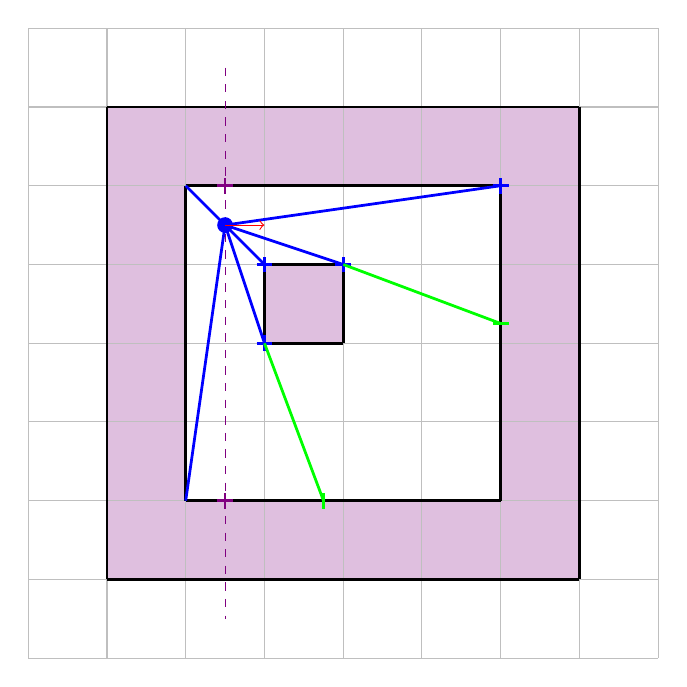
\begin{tikzpicture}
    \fill[violet, opacity=0.25] (1, 1) -- (7, 1) -- (7, 7) -- (1, 7) -- cycle;
    \fill[white] (2, 2) -- (6, 2) -- (6, 6) -- (2, 6) -- cycle;

    \fill[violet, opacity=0.25] (3, 4) -- (4, 4) -- (4, 5) -- (3, 5) -- cycle;

    \draw[color=lightgray] (0, 8) -- (0, 0);
    \draw[color=lightgray] (1, 8) -- (1, 0);
    \draw[color=lightgray] (2, 8) -- (2, 0);
    \draw[color=lightgray] (3, 8) -- (3, 0);
    \draw[color=lightgray] (4, 8) -- (4, 0);
    \draw[color=lightgray] (5, 8) -- (5, 0);
    \draw[color=lightgray] (6, 8) -- (6, 0);
    \draw[color=lightgray] (7, 8) -- (7, 0);
    \draw[color=lightgray] (8, 8) -- (8, 0);

    \draw[color=lightgray] (0, 8) -- (8, 8);
    \draw[color=lightgray] (0, 7) -- (8, 7);
    \draw[color=lightgray] (0, 6) -- (8, 6);
    \draw[color=lightgray] (0, 5) -- (8, 5);
    \draw[color=lightgray] (0, 4) -- (8, 4);
    \draw[color=lightgray] (0, 3) -- (8, 3);
    \draw[color=lightgray] (0, 2) -- (8, 2);
    \draw[color=lightgray] (0, 1) -- (8, 1);   
    \draw[color=lightgray] (0, 0) -- (8, 0);

    \draw[line width=1pt] (1, 1) -- (1, 7);
    \draw[line width=1pt] (1, 1) -- (7, 1);
    \draw[line width=1pt] (7, 1) -- (7, 7);
    \draw[line width=1pt] (1, 7) -- (7, 7);    

    \draw[line width=1pt] (2, 2) -- (2, 6);
    \draw[line width=1pt] (2, 2) -- (6, 2);
    \draw[line width=1pt] (6, 2) -- (6, 6);
    \draw[line width=1pt] (2, 6) -- (6, 6);

    \draw[line width=1pt] (3, 5) -- (4, 5);
    \draw[line width=1pt] (3, 4) -- (4, 4);
    \draw[line width=1pt] (3, 5) -- (3, 4);
    \draw[line width=1pt] (4, 5) -- (4, 4);

    \coordinate (A) at (2.5, 6);
    \coordinate (B) at (6, 6);
    \coordinate (C) at (4, 5);
    \coordinate (D) at (6, 4.25);
    \coordinate (E) at (3, 5);
    \coordinate (F) at (3, 4);
    \coordinate (G) at (3.75, 2);
    \coordinate (H) at (2.5, 2);

    \draw[color=violet, line width=1pt] (2.5, 5.9) -- (2.5, 6.1);
    \draw[color=violet, line width=1pt] (2.4, 6) -- (2.6, 6);

    \draw[color=violet, line width=1pt] (2.5, 1.9) -- (2.5, 2.1);
    \draw[color=violet, line width=1pt] (2.4, 2) -- (2.6, 2);

    \draw[color=blue, line width=1pt] (3, 4.9) -- (3, 5.1);
    \draw[color=blue, line width=1pt] (2.9, 5) -- (3.1, 5);

    \draw[color=blue, line width=1pt] (3, 3.9) -- (3, 4.1);
    \draw[color=blue, line width=1pt] (2.9, 4) -- (3.1, 4);

    \draw[color=blue, line width=1pt] (4, 4.9) -- (4, 5.1);
    \draw[color=blue, line width=1pt] (3.9, 5) -- (4.1, 5);

    \draw[color=blue, line width=1pt] (6, 5.9) -- (6, 6.1);
    \draw[color=blue, line width=1pt] (5.9, 6) -- (6.1, 6);

    \draw[color=green, line width=1pt] (3.75, 1.9) -- (3.75, 2.1);
    \draw[color=green, line width=1pt] (3.74, 2) -- (3.76, 2);

    \draw[color=green, line width=1pt] (6, 4.24) -- (6, 4.26);
    \draw[color=green, line width=1pt] (5.9, 4.25) -- (6.1, 4.25);

    \draw[color=violet, dashed] (2.5, 7.5) -- (A) -- (H) -- (2.5, 0.5);

    \draw[color=green, line width=1pt] (F) -- (G);
    \draw[color=green, line width=1pt] (C) -- (D);

    \draw[color=blue, line width=1pt] (2, 2) -- (2.5, 5.5);
    \draw[color=blue, line width=1pt] (2, 6) -- (2.5, 5.5);
    \draw[color=blue, line width=1pt] (2.5, 5.5) -- (E);
    \draw[color=blue, line width=1pt] (2.5, 5.5) -- (C);
    \draw[color=blue, line width=1pt] (2.5, 5.5) -- (F);
    \draw[color=blue, line width=1pt] (2.5, 5.5) -- (B);

    \fill[color=blue] (2.5, 5.5) circle (0.1);

    \draw[color=red, ->] (2.5, 5.5) -- (3, 5.5);

    % \node[below left] at (A) {A};
    % \node[below right] at (B) {B};
    % \node[above right] at (C) {C};
    % \node[above right] at (D) {D};
    % \node[above left] at (E) {E};
    % \node[above left] at (F) {F};
    % \node[above right] at (G) {G};
    % \node[above left] at (H) {H};
\end{tikzpicture}

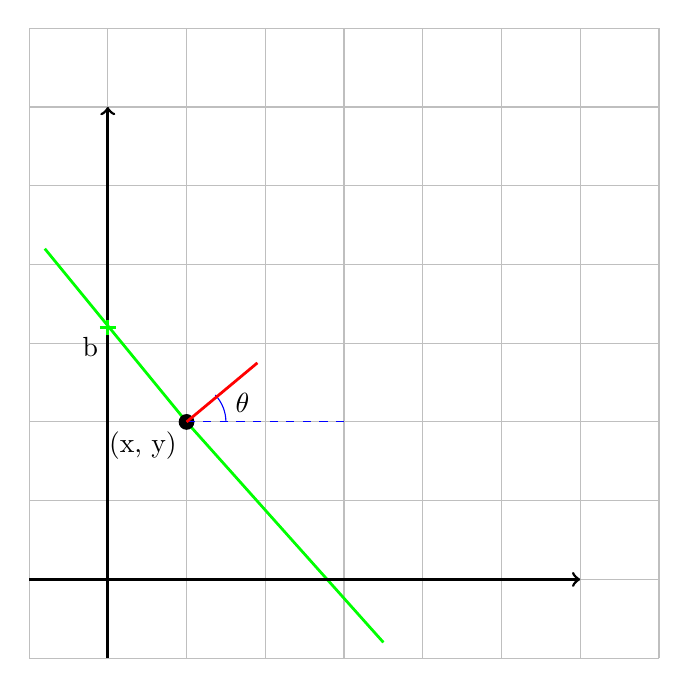
\begin{tikzpicture}

    \draw[color=lightgray] (0, 8) -- (0, 0);
    \draw[color=lightgray] (1, 8) -- (1, 0);
    \draw[color=lightgray] (2, 8) -- (2, 0);
    \draw[color=lightgray] (3, 8) -- (3, 0);
    \draw[color=lightgray] (4, 8) -- (4, 0);
    \draw[color=lightgray] (5, 8) -- (5, 0);
    \draw[color=lightgray] (6, 8) -- (6, 0);
    \draw[color=lightgray] (7, 8) -- (7, 0);
    \draw[color=lightgray] (8, 8) -- (8, 0);

    \draw[color=lightgray] (0, 8) -- (8, 8);
    \draw[color=lightgray] (0, 7) -- (8, 7);
    \draw[color=lightgray] (0, 6) -- (8, 6);
    \draw[color=lightgray] (0, 5) -- (8, 5);
    \draw[color=lightgray] (0, 4) -- (8, 4);
    \draw[color=lightgray] (0, 3) -- (8, 3);
    \draw[color=lightgray] (0, 2) -- (8, 2);
    \draw[color=lightgray] (0, 1) -- (8, 1);   
    \draw[color=lightgray] (0, 0) -- (8, 0);

    \draw[color=green, line width=1pt] (0.2, 5.2) -- (2, 3) -- (4.5, 0.2);

    \draw[line width=1pt, ->] (1, 0) -- (1, 7);
    \draw[line width=1pt, ->] (0, 1) -- (7, 1);

    \draw[color=green, line width=1pt] (1, 4.1) -- (1, 4.3);
    \draw[color=green, line width=1pt] (0.9, 4.2) -- (1.1, 4.2);

    \node[below left] at (1, 4.2) {b};

    \fill[black] (2, 3) circle (0.1);

    \node[below left] at (2, 3) {(x, y)};

    \draw[color=blue, dashed] (2, 3) -- (4, 3);
    \draw[color=blue] (2.5, 3) arc (0:43:0.5);
    \draw[color=red, line width=1pt] (2, 3) -- (2.9, 3.75);
    \node[above right] at (2.5, 3) {$\theta$};
    
\end{tikzpicture}

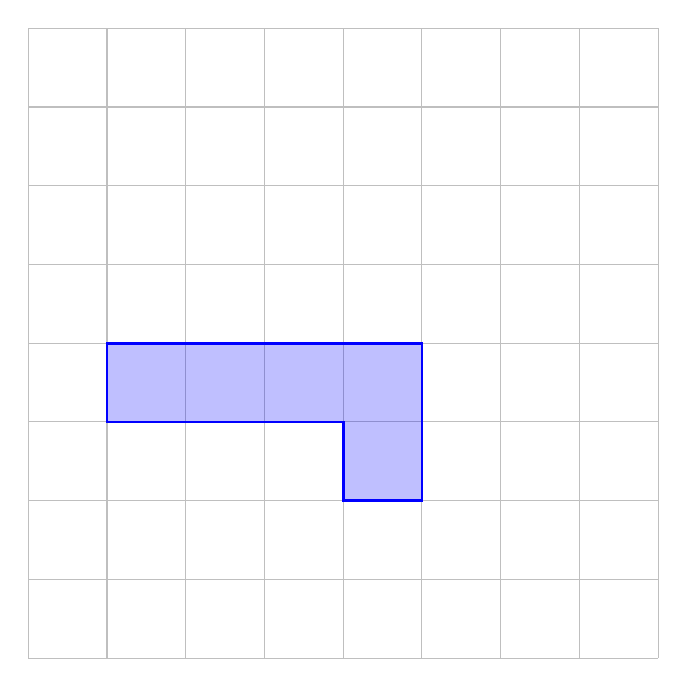
\begin{tikzpicture}

    \draw[color=lightgray] (0, 8) -- (0, 0);
    \draw[color=lightgray] (1, 8) -- (1, 0);
    \draw[color=lightgray] (2, 8) -- (2, 0);
    \draw[color=lightgray] (3, 8) -- (3, 0);
    \draw[color=lightgray] (4, 8) -- (4, 0);
    \draw[color=lightgray] (5, 8) -- (5, 0);
    \draw[color=lightgray] (6, 8) -- (6, 0);
    \draw[color=lightgray] (7, 8) -- (7, 0);
    \draw[color=lightgray] (8, 8) -- (8, 0);

    \draw[color=lightgray] (0, 8) -- (8, 8);
    \draw[color=lightgray] (0, 7) -- (8, 7);
    \draw[color=lightgray] (0, 6) -- (8, 6);
    \draw[color=lightgray] (0, 5) -- (8, 5);
    \draw[color=lightgray] (0, 4) -- (8, 4);
    \draw[color=lightgray] (0, 3) -- (8, 3);
    \draw[color=lightgray] (0, 2) -- (8, 2);
    \draw[color=lightgray] (0, 1) -- (8, 1);   
    \draw[color=lightgray] (0, 0) -- (8, 0);

    \draw[color=blue, line width=1pt] (1, 4) -- (1, 3) -- (4, 3) -- (4, 2) -- (5, 2) -- (5, 4) -- cycle;
    \fill[color=blue, opacity=0.25] (1, 4) -- (1, 3) -- (4, 3) -- (4, 2) -- (5, 2) -- (5, 4) -- cycle;
 
    
    
\end{tikzpicture}



\end{document}